\documentclass{beamer}
\usepackage[utf8]{inputenc}

\usetheme{Madrid}

%% ADDITIONAL NICOLÁS
\usepackage{ragged2e}
\usepackage{amssymb}
\usepackage{subcaption}

\usefonttheme{serif}
\definecolor{UBCblue}{rgb}{0.01569, 0.11765, 0.25882} % PSU Blue
\usecolortheme[named=UBCblue]{structure}

%% ADDITIONAL NICOLÁS




%------------------------------------------------------------
%This block of code defines the information to appear in the
%Title page
\title[Weekly Reports] %optional
{PhD in Energy and Mineral Engineering at PSU}

\subtitle{Nicolás's Research - Reports}

\author[Nicolás Bueno] % (optional)
{Nicolás Bueno\inst{1} \and Advisor: Dr. Ayala\inst{1}}

\institute[EME] % (optional)
{
	\inst{1}%
	Department of Energy and Mineral Engineering\\
	Penn State University\\
	
\includegraphics[height=1cm]{pics/PSU_EMS.png}
}

\date[Fall 2021] % (optional)
{}

%\logo{
\includegraphics[height=1cm]{pics/PSU_EMS.png}}

%End of title page configuration block
%------------------------------------------------------------



%------------------------------------------------------------
%The next block of commands puts the table of contents at the 
%beginning of each section and highlights the current section:

\AtBeginSection[]
{
	\begin{frame}
		\frametitle{Table of Contents}
		\tableofcontents[currentsection]
	\end{frame}
}
%------------------------------------------------------------


\begin{document}
	
	%The next statement creates the title page.
	\frame{\titlepage}
	
	%---------------------------------------------------------
	%This block of code is for the table of contents after
	%the title page
	\begin{frame}
		\frametitle{Table of Contents}
		\tableofcontents
	\end{frame}
	%---------------------------------------------------------
	
	\justifying
	\section{Spring 2022}
	
	\subsection{Report Jan 24 - 2022}
	\label{}
	\justifying
	\begin{frame}
		\textbf{Report Jan 24 - 2022}\\~\\
		Main discussion points:
		\begin{itemize}
			\item Cheng's paper
			\item LBM Code state
			\item Short-term Medium-term objectives
		\end{itemize}
	\end{frame}
	
	\begin{frame}{Cheng's paper}
		Bulk equation for the Shan-Chen force:
		\begin{equation*}
		\mathbf{F} = -G \psi(x) \sum_i \omega_i \psi(x+\mathbf{c}_i \delta t) \mathbf{c}_i \, \, \, \, \, \psi := \sqrt{\frac{2(P^{\text{\tiny EoS}}-c_s^2\rho)}{G \delta t c_s^2}}
		\end{equation*}
		\begin{itemize}
			\item MRT model
			\item Multi-component partially miscible
		\end{itemize}
	\end{frame}
	
	\begin{frame}{LBM state}
		This I advanced before last state:
		\begin{itemize}
			\item Tried the binary printing (unsuccessful)
			\item Run the single component multi-phase model (successful)
			\item Equation to count the number of molecules in a lattice. 
			\item Short-term mid-term objectives
		\end{itemize}
	\end{frame}

	\begin{frame}{van der Waals validation}
		\begin{figure}
			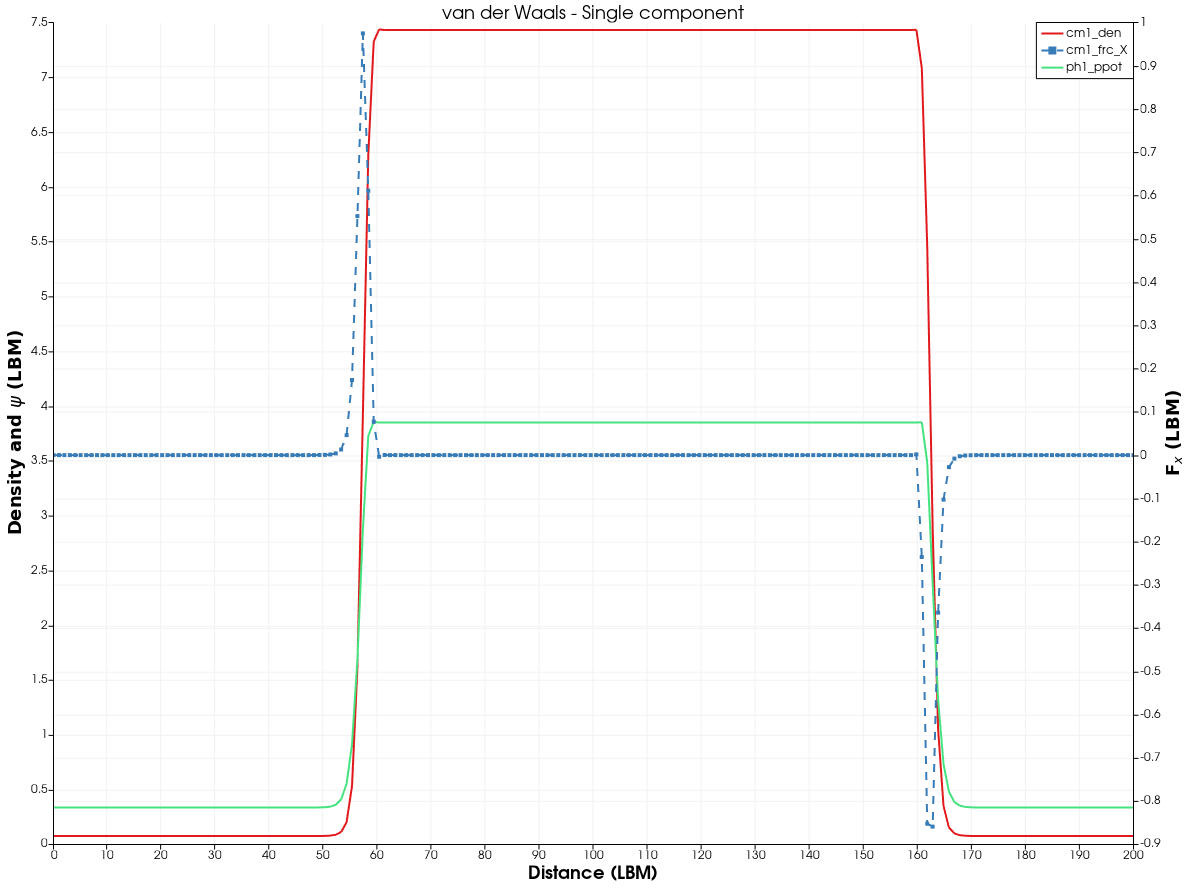
\includegraphics[scale=0.2]{pics/vdwValidation.png}
		\end{figure}
	\end{frame}

	\begin{frame}{Peng Robinson validation}
		\begin{columns}
			\column{0.4\textwidth}
			\begin{figure}
				\centering
				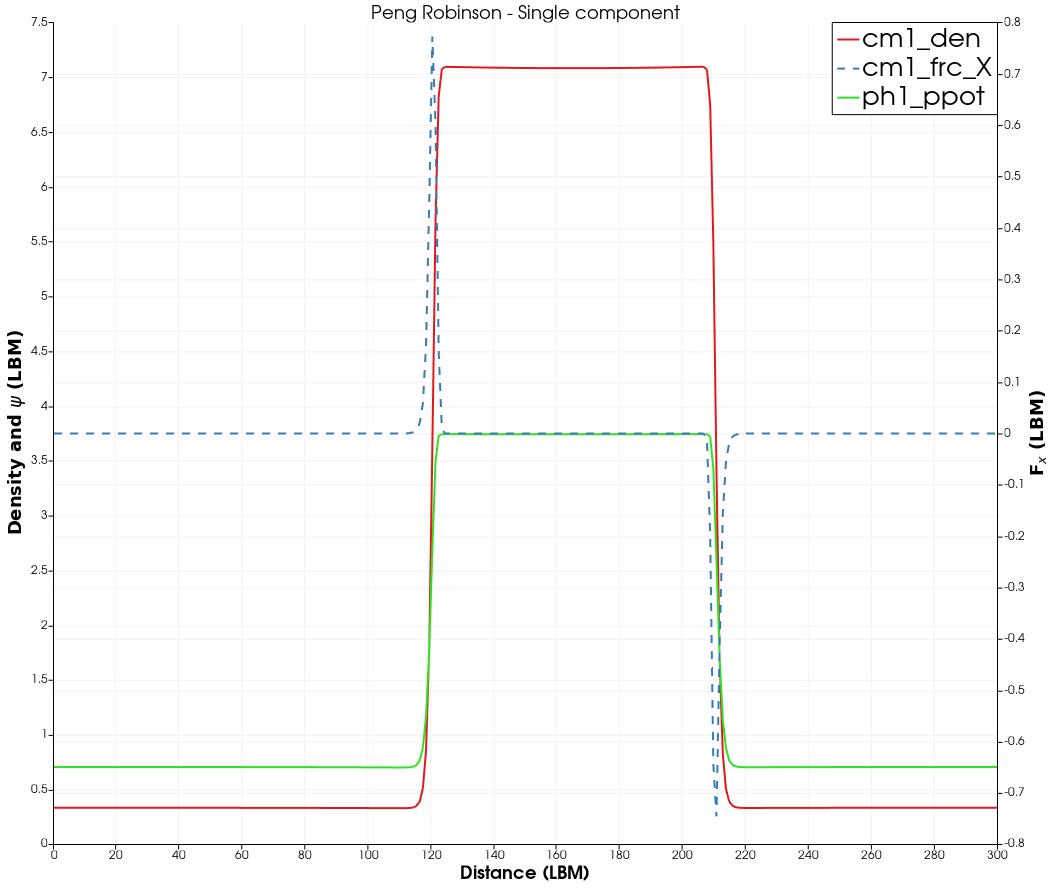
\includegraphics[scale=0.12]{pics/prValidation.png}
				\caption{}   
			\end{figure}
			\column{0.4\textwidth}
			\begin{figure}
				\centering
				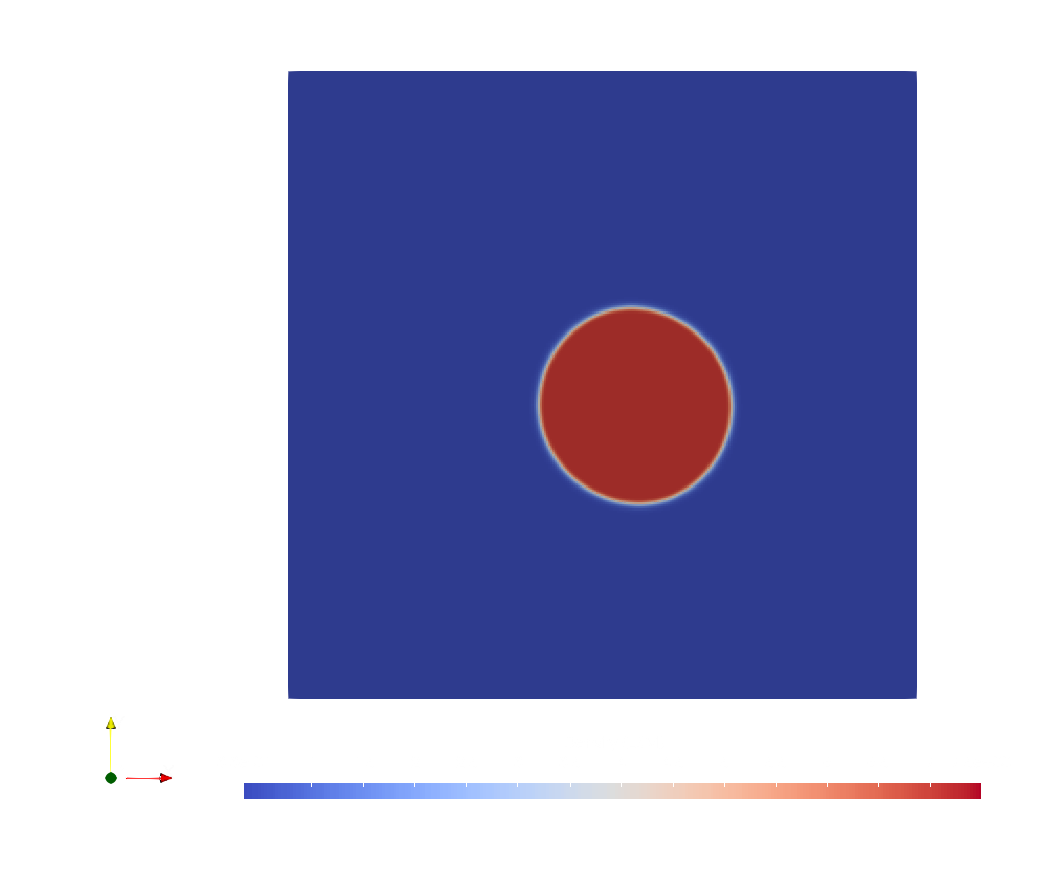
\includegraphics[scale=0.15]{pics/prValidation2.png}
			\end{figure}
		\end{columns}
	\end{frame}

	\begin{frame}{Where I am going?}
		I was rediscovering the concept of $\psi$ that now belongs to the bulk (phase) entity. In Kruger's book is assigned to each component, so each components computes its own SC force. Other forces split according to $\rho_i$.\\
		Two components structure is ready to start building the 2-component case that Cheng uses for validation. 
	\end{frame}
	\begin{frame}{Actions}
		\begin{itemize}
			\item Dry-run of research proposal for qualifying exam.Deep dive into literature looking for problems in current problems and interesting applications (reactions-solute transport-energy-multiphase).
			\item LBM tutorials is the next short-term project
			\item Finish my own code to run the Cheng's cases in our simulator. 
			\item Long-term: evaluate the Kruger's perspective of calculating SC per component.
		\end{itemize}
	\end{frame}
	
	%---------------------------------------------------------
	%---------------------------------------------------------
	\subsection{Meeting with LBM questions}
	\label{}
	\justifying
	\begin{frame}
		\textbf{Meeting with LBM questions}\\~\\
		Questions:
		\begin{itemize}
			\item LBM Formulation
			\begin{itemize}
				\item Are the equations molar/mass based? Which one should it be for efficiency?
			\end{itemize}
			\item Boundary conditions
			\begin{itemize}
				\item Composition for pressure BC at outlet or inlet
			\end{itemize}
		\end{itemize}
	\end{frame}
	
	%---------------------------------------------------------
	%---------------------------------------------------------
	
	%---------------------------------------------------------
	%---------------------------------------------------------
	%---------------------------------------------------------
	%---------------------------------------------------------
	%---------------------------------------------------------
	%---------------------------------------------------------
	%---------------------------------------------------------
	%---------------------------------------------------------
	%---------------------------------------------------------
	
	\begin{frame}{Present}
		Present...
	\end{frame}
	
	\section*{Useful frame options}
	%---------------------------------------------------------
	\begin{frame}
		\textbf{Report XXX XX - 202X}\\~\\
		Main discussion points:
		\begin{itemize}
			\item Topic 1
			\item Topic 2
		\end{itemize}
	\end{frame}
	%---------------------------------------------------------

	%---------------------------------------------------------
	\begin{frame}
	\end{frame}
	%---------------------------------------------------------
	%---------------------------------------------------------
	\begin{frame}
	\end{frame}
	%---------------------------------------------------------
	%---------------------------------------------------------
	\begin{frame}
	\end{frame}
	%---------------------------------------------------------
		%---------------------------------------------------------
	%Changing visivility of the text
	\begin{frame}
		\frametitle{Sample frame title}
		This is a text in second frame. For the sake of showing an example.
		
		\begin{itemize}
			\item<1-> Text visible on slide 1
			\item<2-> Text visible on slide 2
			\item<3> Text visible on slides 3
			\item<4-> Text visible on slide 4
		\end{itemize}
	\end{frame}
	
	%---------------------------------------------------------
	
	
	%---------------------------------------------------------
	%Example of the \pause command
	\begin{frame}
		In this slide \pause
		
		the text will be partially visible \pause
		
		And finally everything will be there
	\end{frame}
	%---------------------------------------------------------
	
	%---------------------------------------------------------
	%Highlighting text
	\begin{frame}
		\frametitle{Sample frame title}
		
		In this slide, some important text will be
		\alert{highlighted} because it's important.
		Please, don't abuse it.
		
		\begin{block}{Remark}
			Sample text
		\end{block}
		
		\begin{alertblock}{Important theorem}
			Sample text in red box
		\end{alertblock}
		
		\begin{examples}
			Sample text in green box. The title of the block is ``Examples".
		\end{examples}
	\end{frame}
	%---------------------------------------------------------
	
	
	%---------------------------------------------------------
	%Two columns
	\begin{frame}
		\frametitle{Two-column slide}
		
		\begin{columns}
			
			\column{0.5\textwidth}
			This is a text in first column.
			$$E=mc^2$$
			\begin{itemize}
				\item First item
				\item Second item
			\end{itemize}
			
			\column{0.5\textwidth}
			This text will be in the second column
			and on a second tought this is a nice looking
			layout in some cases.
		\end{columns}
	\end{frame}
	%---------------------------------------------------------
	
	
\end{document}